\documentclass{ctexart}
\usepackage{amsmath}
\usepackage{float}
\usepackage{amssymb}
\usepackage{graphicx}
\usepackage{gbt7714}
\usepackage{pifont}
\usepackage{wrapfig}
\usepackage{multirow}
\usepackage{array}

\ctexset{
    % 修改 section。
    section={   
        name={,、},
        number={\chinese{section}}
    }
}

\title{偏振光的观察与测量}
\author{陆知辰-10225301478}
\date{\today}
\graphicspath{{figure/}}

\begin{document}

\begin{titlepage}
  \centering
  % 插入图片
  
\includegraphics[width=0.5\textwidth]{ecnu.png}
  
  % 空行用于调整标题位置
  \vspace*{\baselineskip}
  
  % 标题
  \Huge\textbf{物\quad 理\quad 实\quad 验 \quad (二)}
  % 空行用于调整标题和其他信息之间的间距
  \vspace*{0.3\baselineskip}
  
  % 具体实验名称
  \huge 偏振光的观察与测量
  
  % 空行用于调整时间和其他信息之间的间距
  \vspace*{2\baselineskip}
  
  % 时间
  \large 时间:\today
  
  % 空行用于调整时间和其他信息之间的间距
  \vspace*{\baselineskip}
  
  % 创作人
  \large 创作人:陆知辰
  
  % 空行用于调整创作人和学号之间的间距
  \vspace*{\baselineskip}
  
  % 学号
  \large 学号:10225301478
  
\end{titlepage}
\newpage
\tableofcontents
\newpage
\section{实验摘要}
  \subsection{实验概要}
  光的偏振现象不仅进一步验证了光具有波动性,而且验证了光是一种横波,光的偏振现象的研究,
  使人们对光的传播规律有了新的认识,利用光的偏振性所开发出来的各种偏振光元件、偏振光仪器和偏振光技术在光调制器、
  光开关、光学计量、应力分析、光信息处理、光通信、激光和光电子学器件等方面都有着广泛的应用,在现代科学技术中发挥了极其重要的作用。

  \subsection{实验目的}
  1.\quad 了解和掌握线偏振光、圆偏振光、椭圆偏振光的产生及检验方法。

  2.\quad 了解和掌握1/4波片、1/2波片和偏振片的作用和应用。

  3.\quad 验证马吕斯定律。

\section{实验原理}
  \subsection{偏振光的种类}
  光是电磁波,它的电矢量和磁矢量相互垂直,且又垂直于光的传播方向,
  通常用电矢量代表光矢量,并将光矢量和光的传播方向所构成的平面称为光的振动面.按光矢量的不同振动状态,
  可以把光分为五种偏振态,如图37.1所示.如在垂直于传播方向内,光矢量的方向是任意的,且各个方向的振幅相等,
  则称为自然光;如光矢量沿着一个固定方向振动,则称为线偏振光或平面偏振光;如果有的方向光矢量振幅较大,有的方向光矢量振幅较小,
  则称为部分偏振光;如果光矢量的大小和方向随时间作周期性变化,
  且光矢量的末端在垂直于光传播方向的平面内的轨迹是圆或椭圆,则分别称为圆偏振光或椭圆偏振光。

  \subsection{线偏振光的产生}
  根据布儒斯特定律,如图\ref{pianzhentai}所示,

  \begin{figure}[H]\label{pianzhentai}
    \centering
    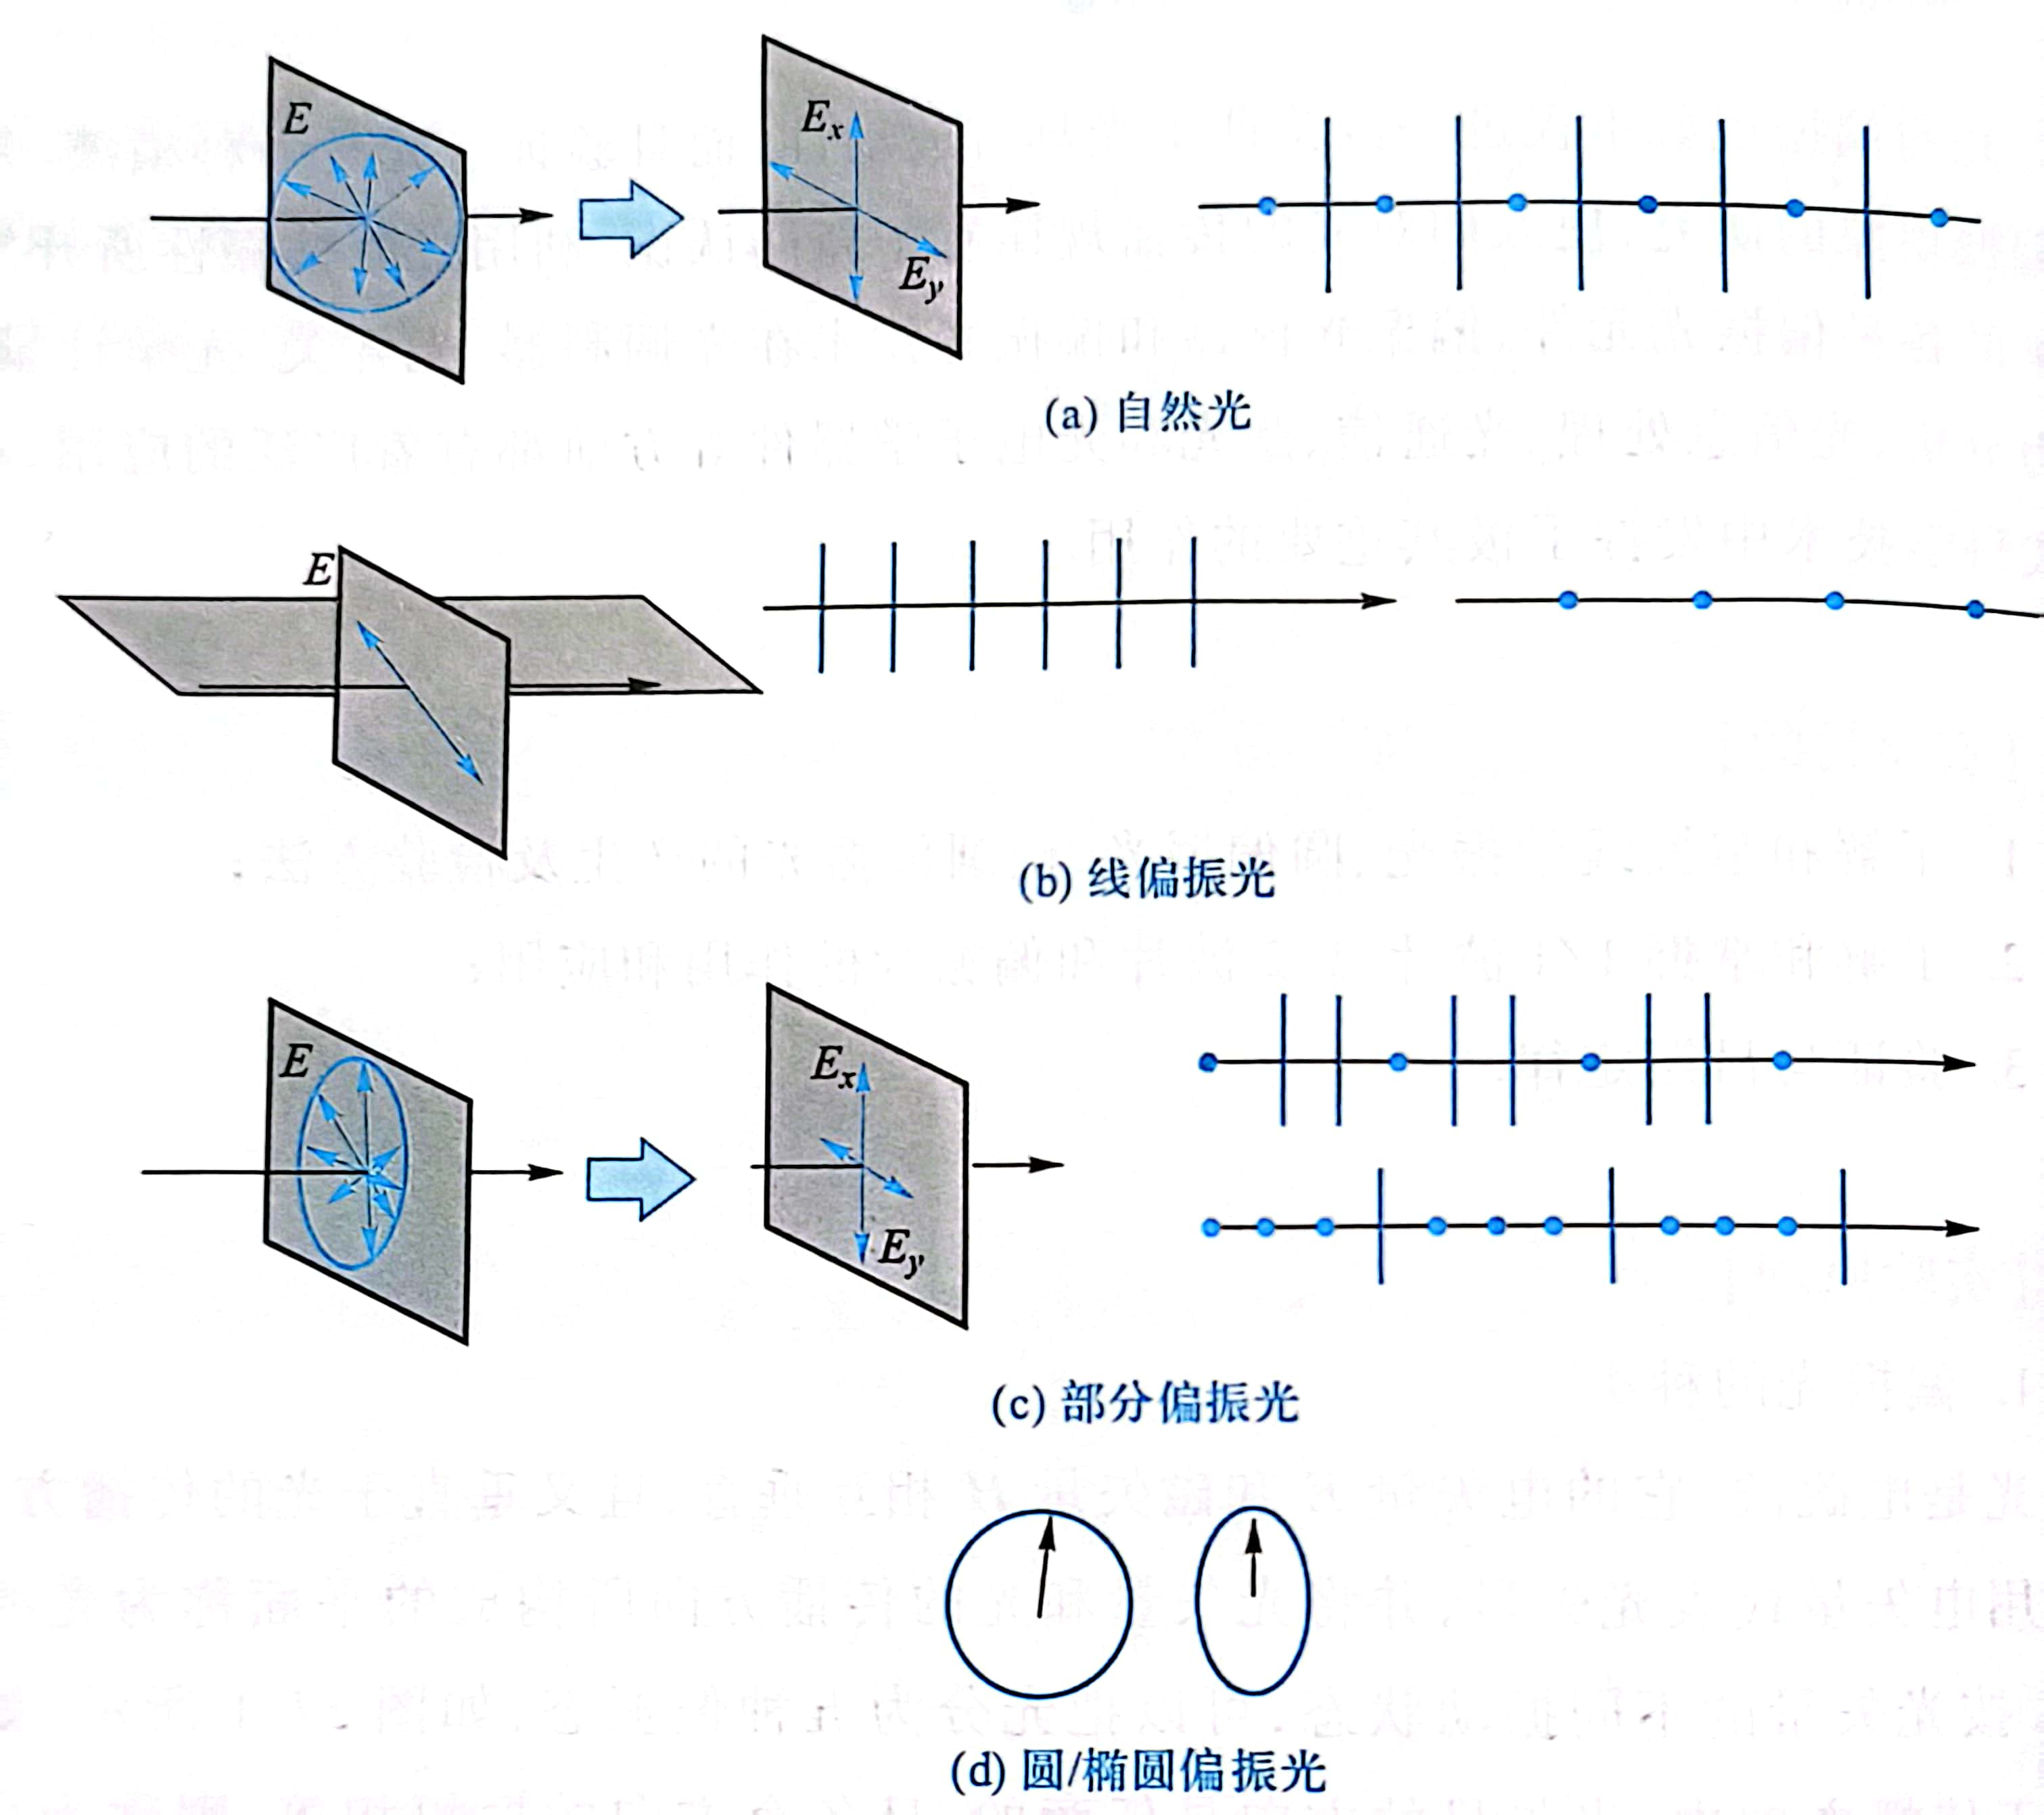
\includegraphics[width=0.7\textwidth,height=0.4\textheight]{pianzhentai.jpg}
    \caption{偏振光五种形态}
  \end{figure}
  

  当自然光以$i_{b} = \arctan (\frac{n_{2}}{n_{1}})$
  的人射角从折射率为$n_{1}$的空气入射至折射率为$n_{2}$的介质表面上时,
  其反射光为完全的线偏振光,振动面垂直于人射面;而透射光为部分偏振光,此时我们称$i_{b}$为布儒斯特角。
  如果自然光以i入射到一叠平行玻璃片堆上,则经过多次反射和折射,最后从玻璃片堆透射出来的光也接近于线偏振光,
  如图\ref{pianzhenguangchansheng}所示.

  \begin{figure}[H]\label{pianzhenguangchansheng}
    \centering
    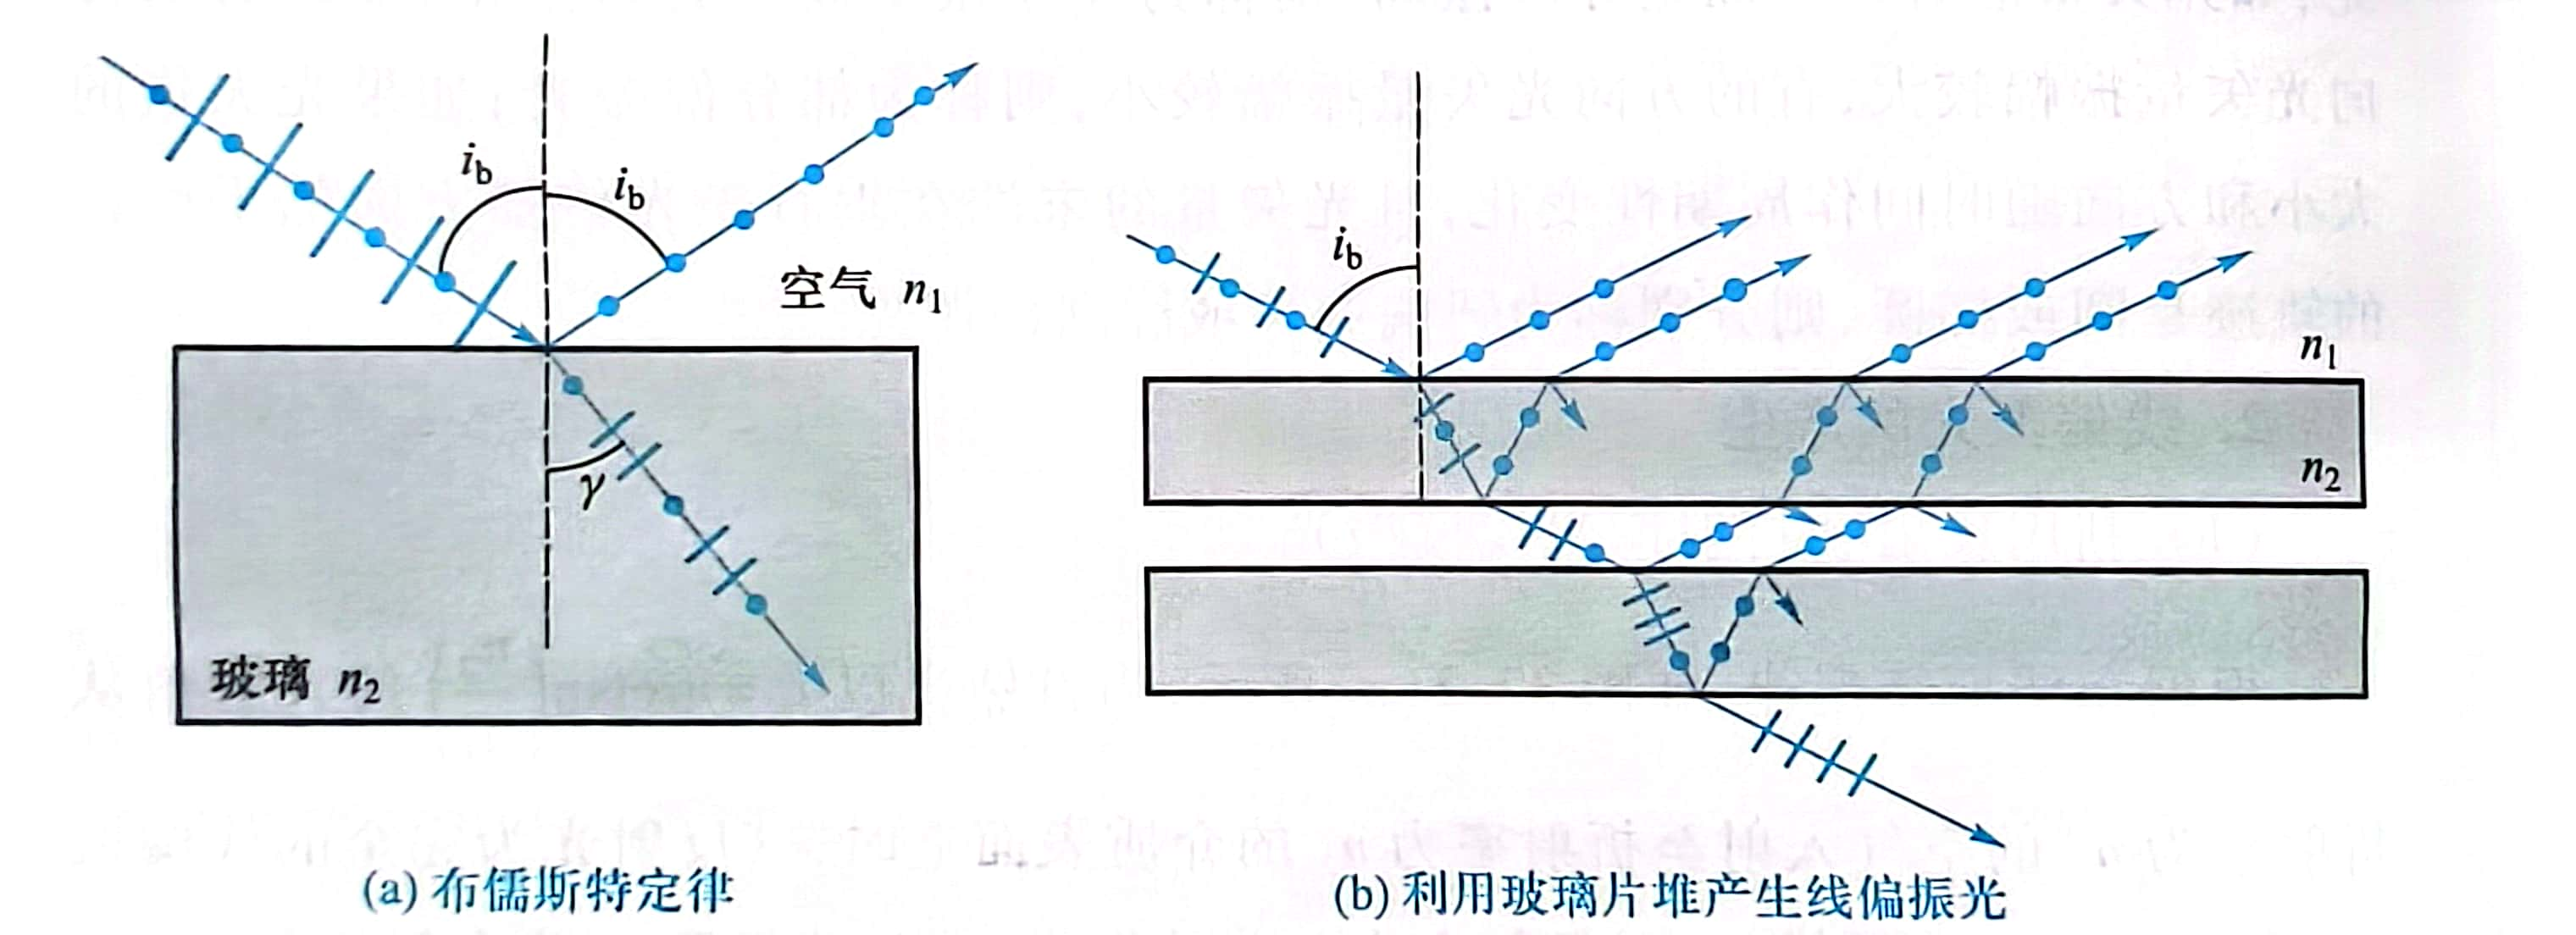
\includegraphics[width=0.7\textwidth,height=0.2\textheight]{pianzhengguangchansheng.jpg}
    \caption{偏振光的产生}
  \end{figure}

  \subsection{利用偏振片获得线偏振光}
  偏振片是利用某些有机化合物晶体的“二向色性“制成的,当自然光通过这种偏振片后,
  光矢量垂直于偏振片透振方向的分量几乎完全被吸收,光矢量平行于透振方向的分量几乎完全通过,因此透射光基本上为线偏振光。

  \subsection{波晶片的分类}
  波晶片简称波片,它通常是一块光轴平行于表面的单轴晶片,一束平面偏振光垂直入射到波晶片后,
  便分解为振动方向与光轴方向平行的e光和振动方向与光轴方向垂直的。光两部分,这两种光在晶体内的传播方向虽然一致,
  但它们在晶体内传播的速度却不相同,于是e光和o光通过波晶片后就产生固定的相位差$\delta$,
  即$\delta = \frac{2\pi}{\lambda} (n_{o} - n_{e}) l$,式中$\lambda$为人射光的波长,l为品片的厚度,$n_{o},n_{e}$分别为o光和e光的主折射率。

  某种单色光经过波晶片后,若e光和o光产生的相位差为$\delta=(2k+1)\pi/2$,
  则此波晶片称为该单色光的1/4波片;若e光和o光产生的相位差为$\delta=(2k+1)\pi$,则此波晶片称为该单色光的1/2波片;
  能产生相位差为$\delta=2k\pi$的波晶片,称为全波片。

  通常波片用云母片剥离成适当厚度或用石英晶体研磨成薄片,由于石英晶体是正晶体,
  其o光比e光的速度快,沿光轴方向振动的光(e光)传播速度慢,
  故光轴称为慢轴,与之垂直的方向称为快轴,对于负品体制成的波片,光轴就是快轴。

  \subsection{平面偏振光通过各种波片后偏振态的改变}
  一束振动方向与光轴成$\theta$角的平面偏振光垂直入射到波片后,会产生振动方向相互垂直的e光和o光,
  如图\ref{bojingpianguanglu}所示,
  其E矢量大小分别为$E_{e} = E \cos \theta$、$E_{o}=E\sin\theta$.通过波片后,
  二者产生一附加相位差.离开波片时合成波的偏振性质决定于相位差$\delta$和$\theta$.
  如果入射偏振光的振动方向与波片的光轴夹角为0或$\pi/2$,
  则任何波片对它都不起作用,即从波片出射的光仍为原来的线偏振光.而如果不为0或$\pi/2$,那么线偏振光通过1/2波片后,
  出来的也仍为线偏振光,但它振动方向将旋转$2\theta$,
  即出射光和入射光的电矢量对称于光轴;线偏振光通过1/4波片后,则可能产生线偏振光、
  圆偏振光和长轴与光轴垂直或平行的椭圆偏振光,这取决于人射线偏振光振动方向与光轴的夹角$\theta$。

  \begin{figure}[H]\label{bojingpianguanglu}
    \centering
    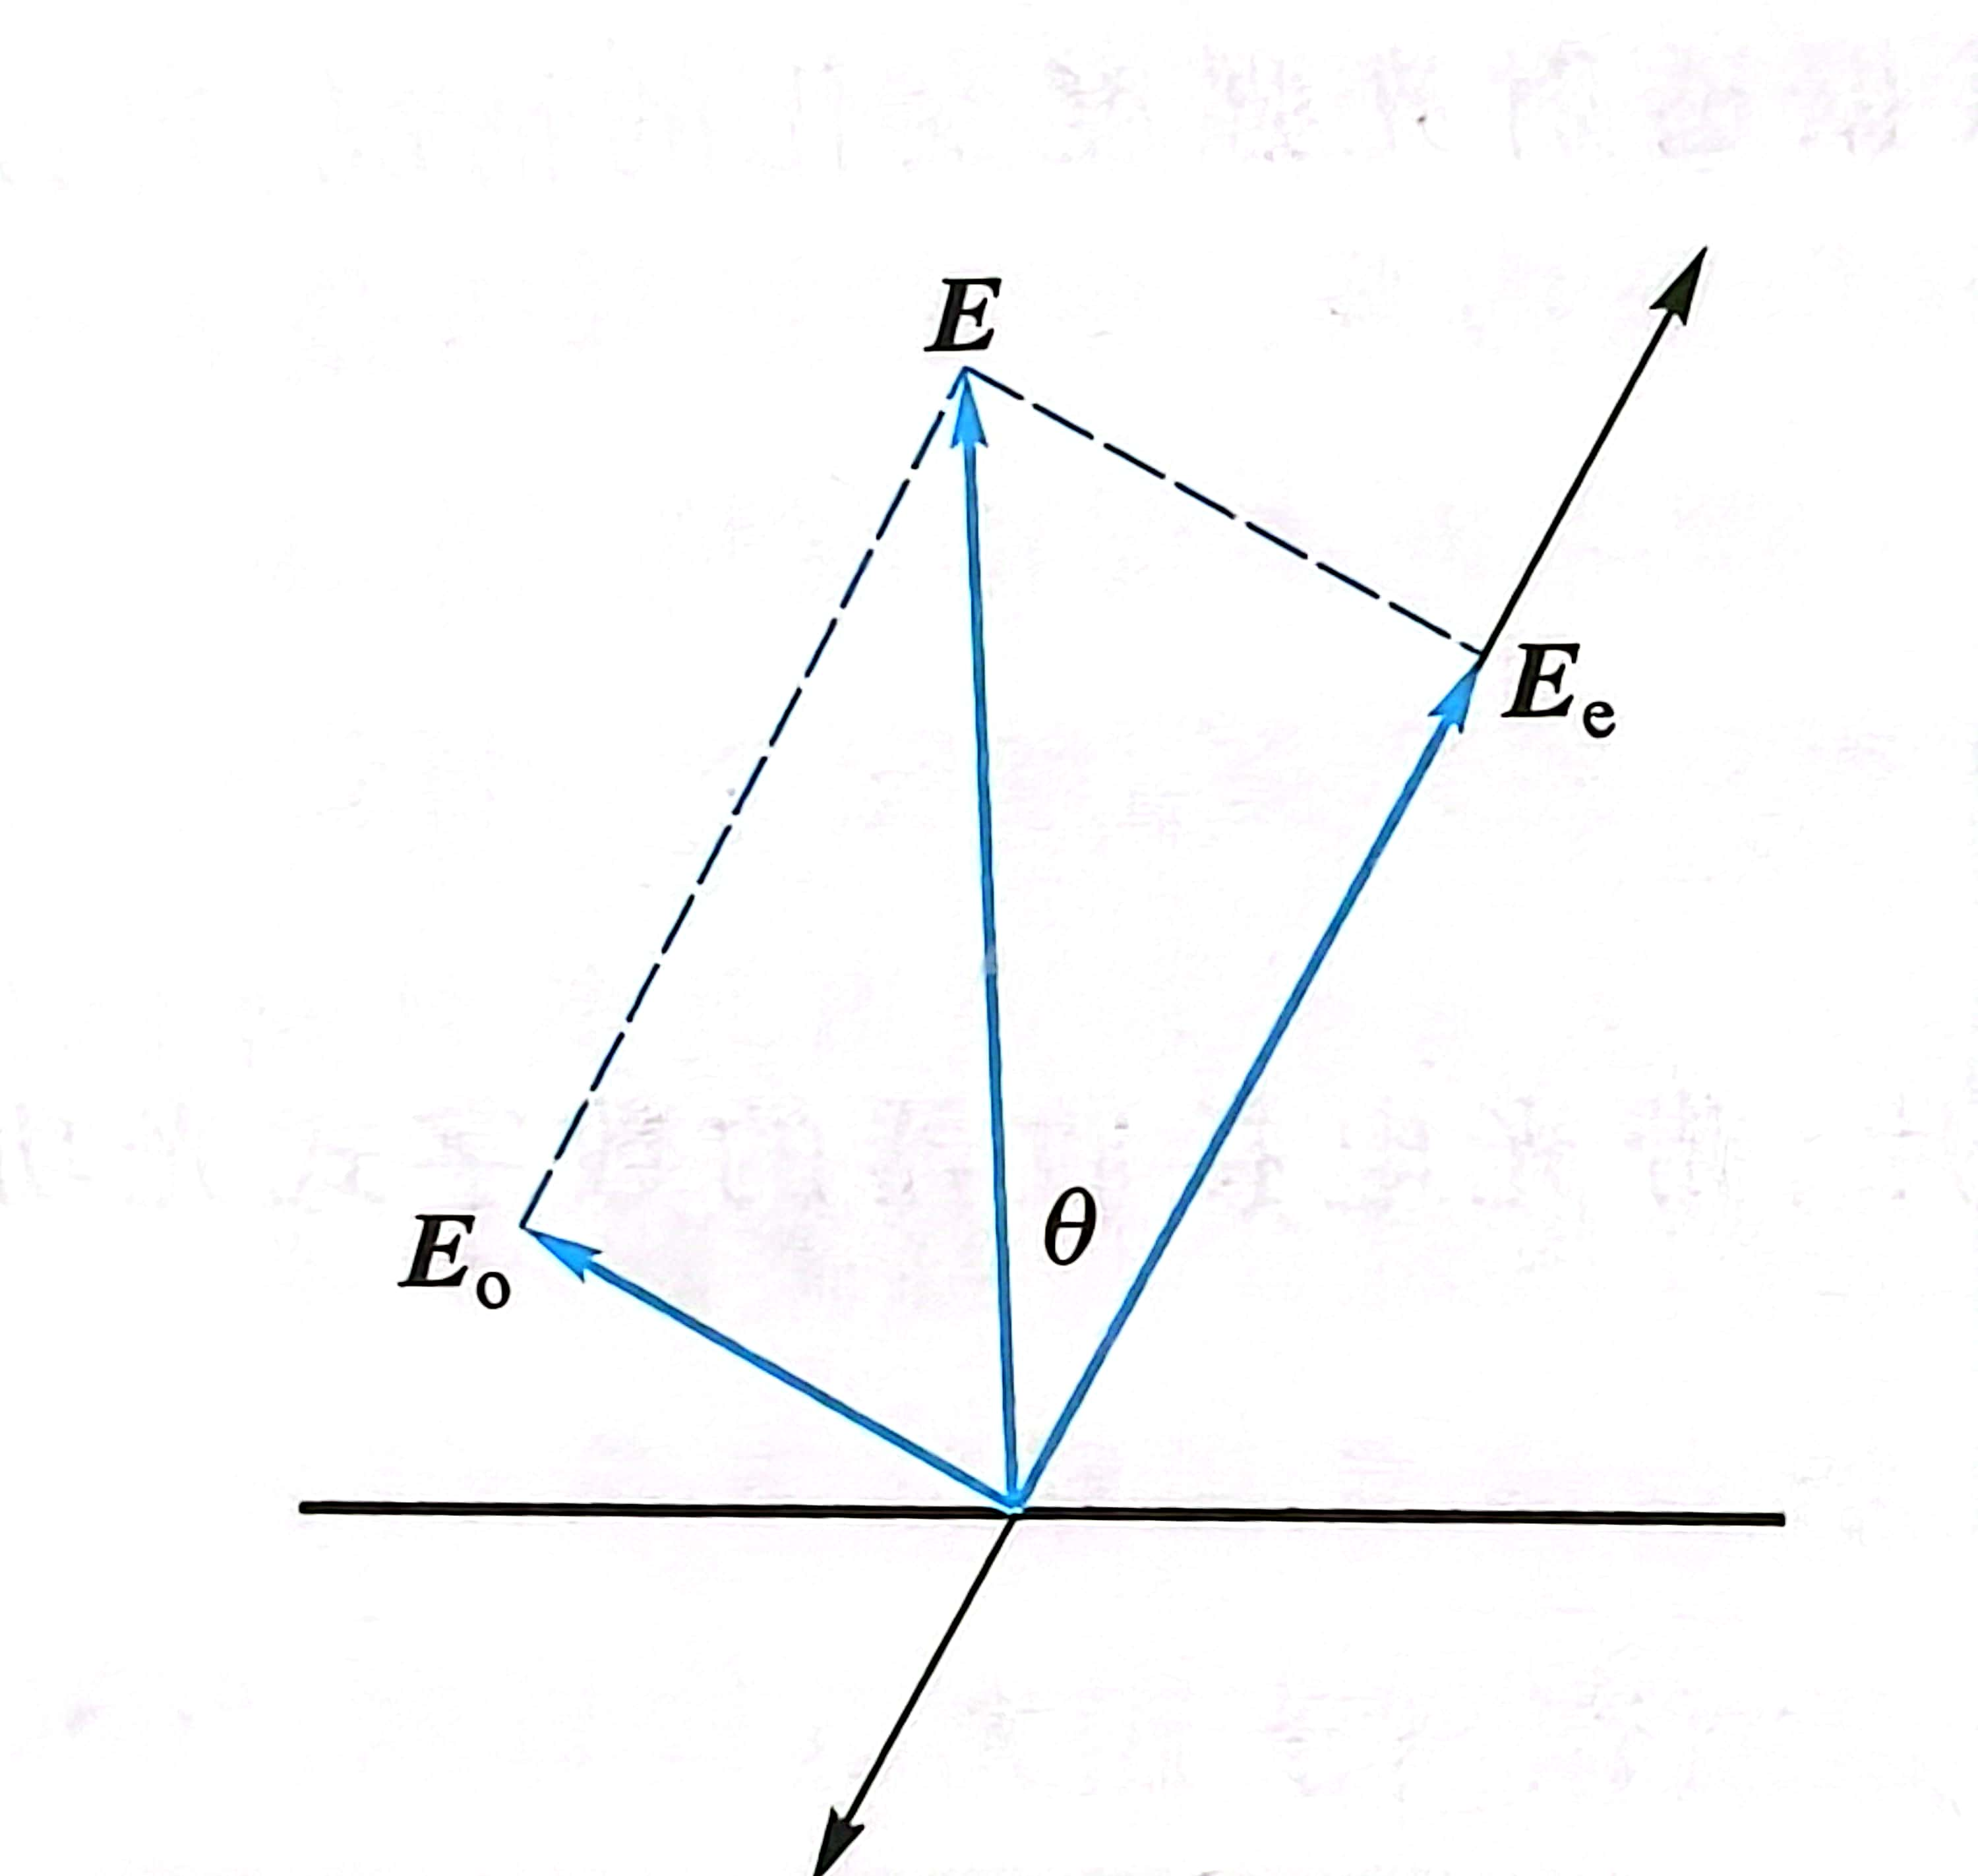
\includegraphics[width=0.5\textwidth,height=0.3\textheight]{bojingpianguanglu.jpg}
    \caption{线偏振光经过波片后的光路示意图}
  \end{figure}

  \subsection{偏振光的鉴别}
  鉴别入射光的偏振态须借助于检偏器(即偏振片)和1/4波片:使入射光通过检偏器后,检测其透射光强并转动检偏器,
  如图\ref{jianbiefangfa}所示.

  \begin{figure}[H]\label{jianbiefangfa}
    \centering
    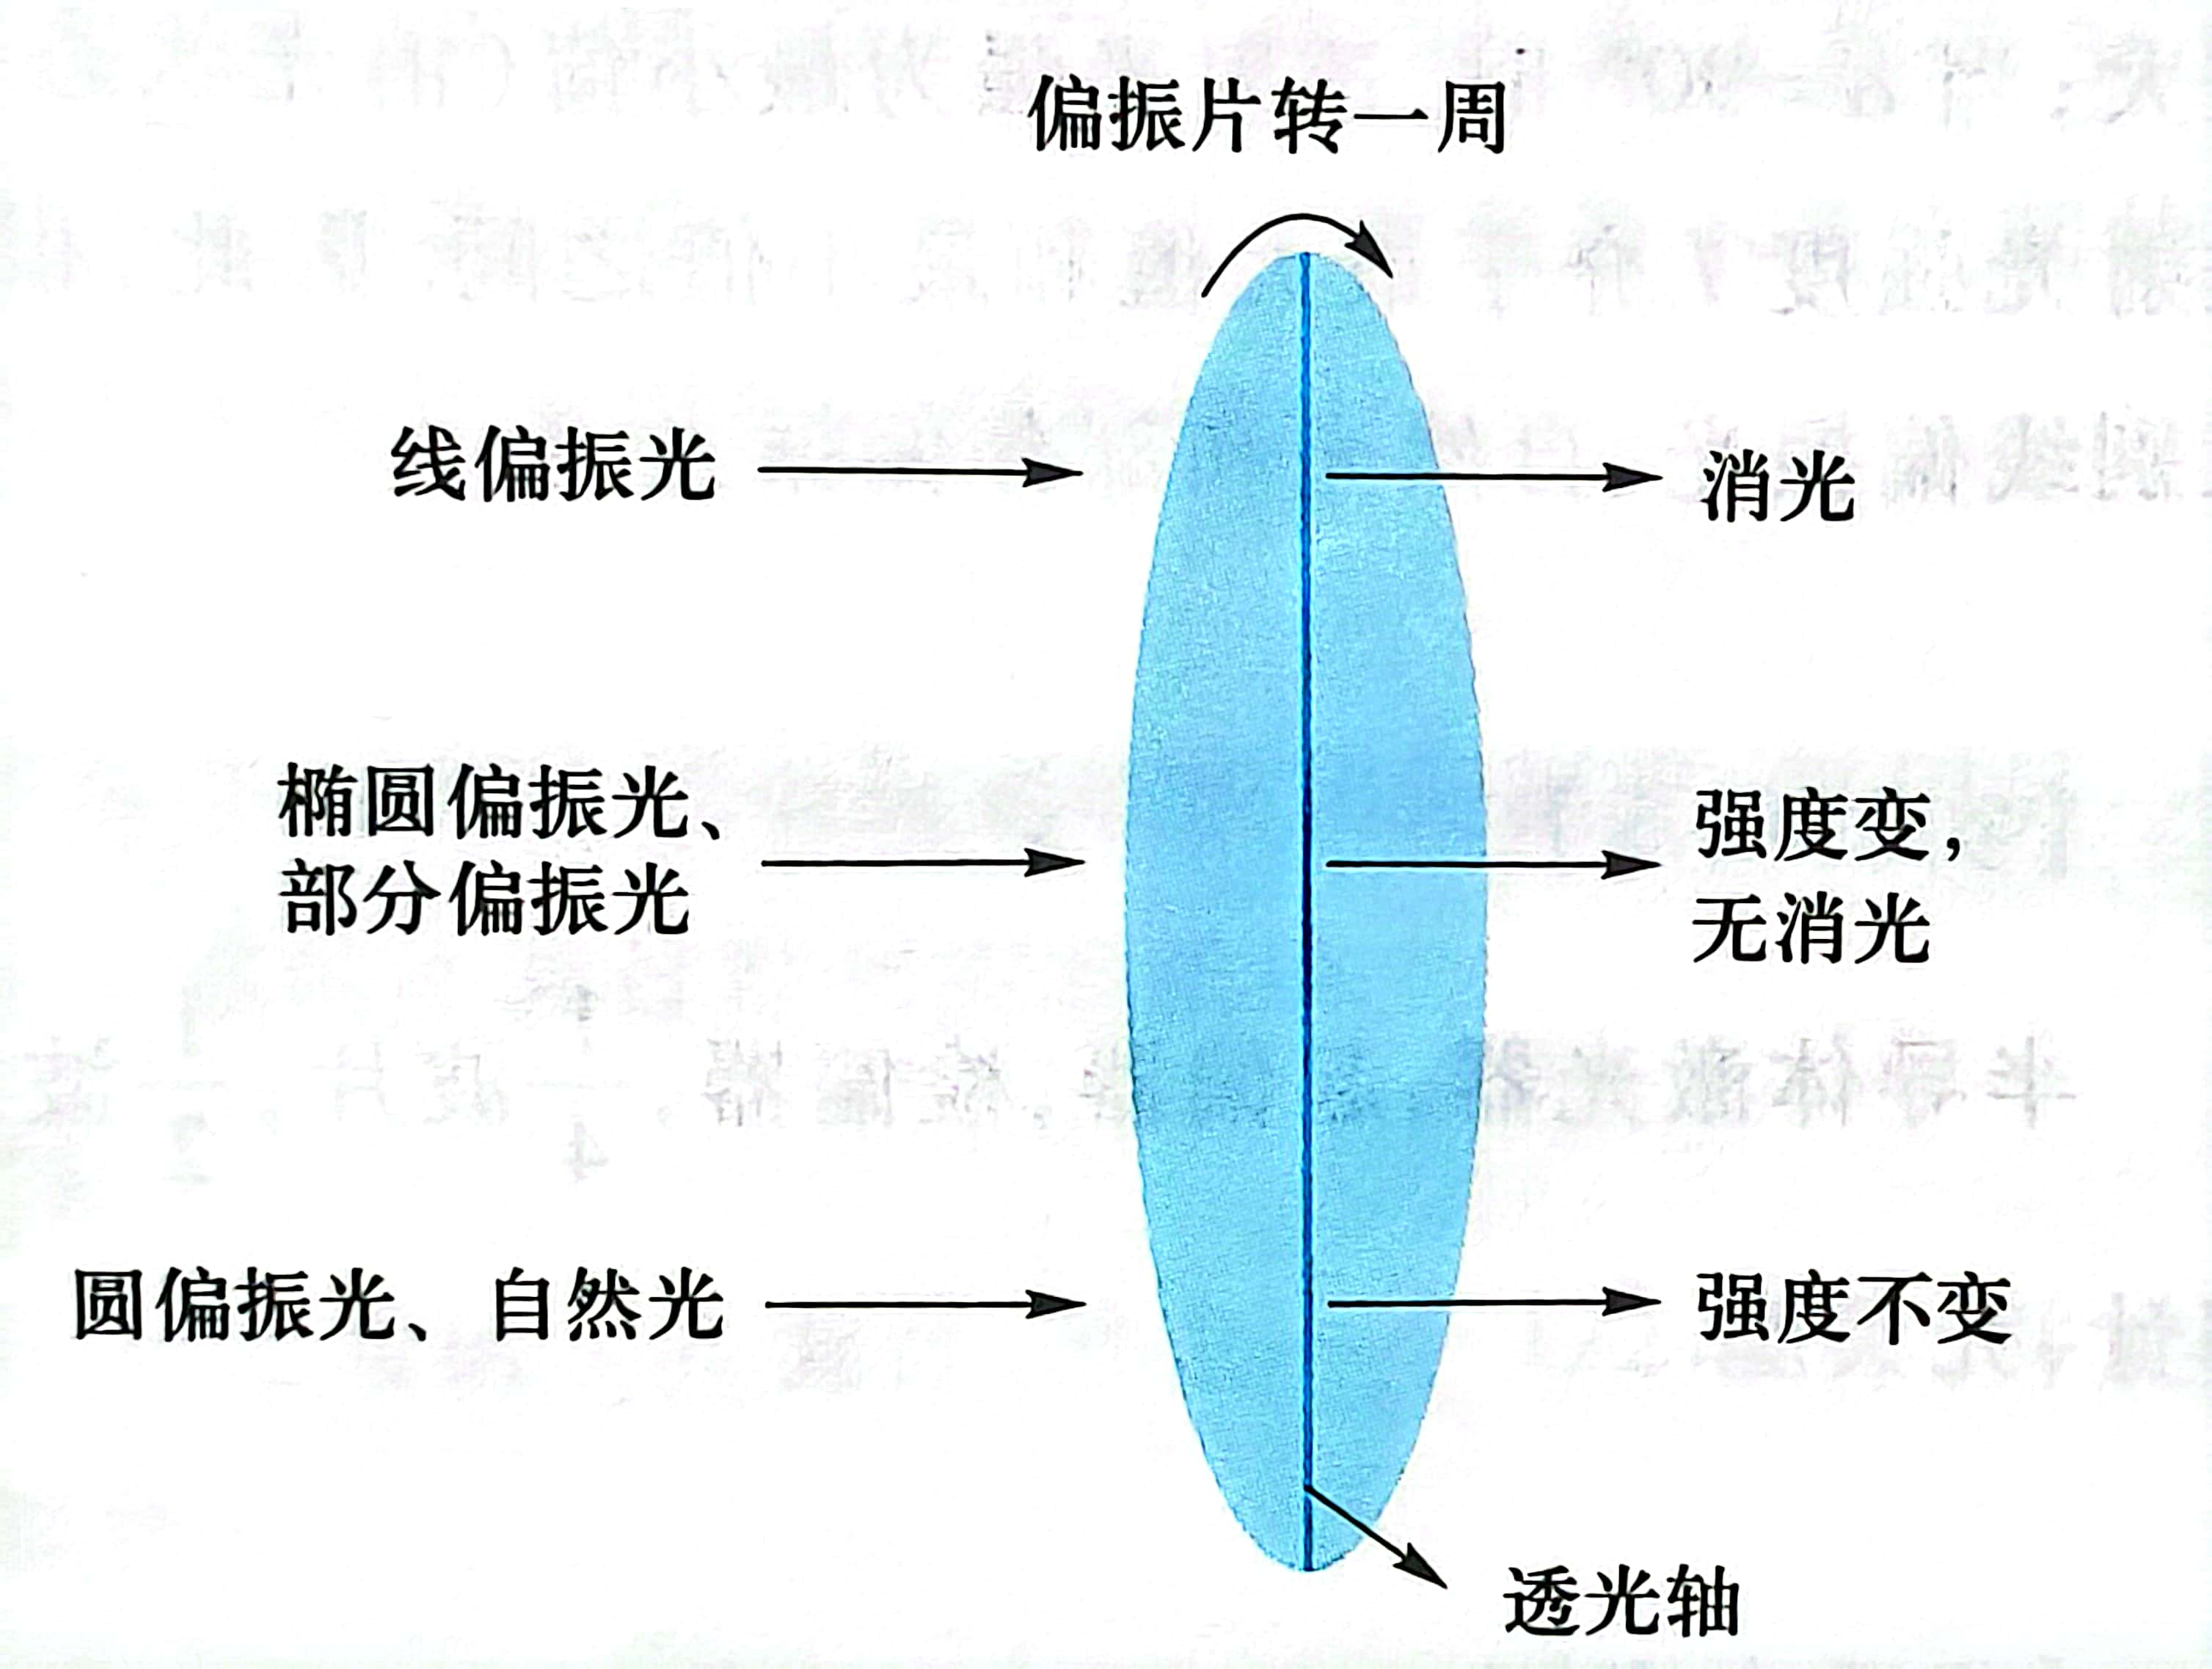
\includegraphics[width=0.4\textwidth,height=0.3\textheight]{jianbiefangfa.jpg}
    \caption{鉴别偏振光方法示意图1}
  \end{figure}

  若转动检偏器,出现透射光强为零(称“消光”)的现象,则入射光必为线偏振光。
  
  若转动检偏器,透射光的强度没有变化,则可能为自然光或圆偏振光(或两者的混合)。

  若转动检偏器,透射光强虽有变化但不出现消光现象,则入射光可能是椭圆偏振光或部分偏振光。

  要进一步作出鉴别,则需在入射光与检偏器之间插入一块1/4波片,如图\ref{jinyibujianbie}所示,若人射光是圆偏振光,
  则通过1/4波片后将变成线偏振光,当1/4波片的慢轴(或快轴)与被检测的椭圆偏振光的长轴或短轴平行时,
  透射光也为线偏振光,于是转动检偏器也会出现消光现象;否则,就是部分偏振光.

  \begin{figure}[H]\label{jinyibujianbie}
    \centering
    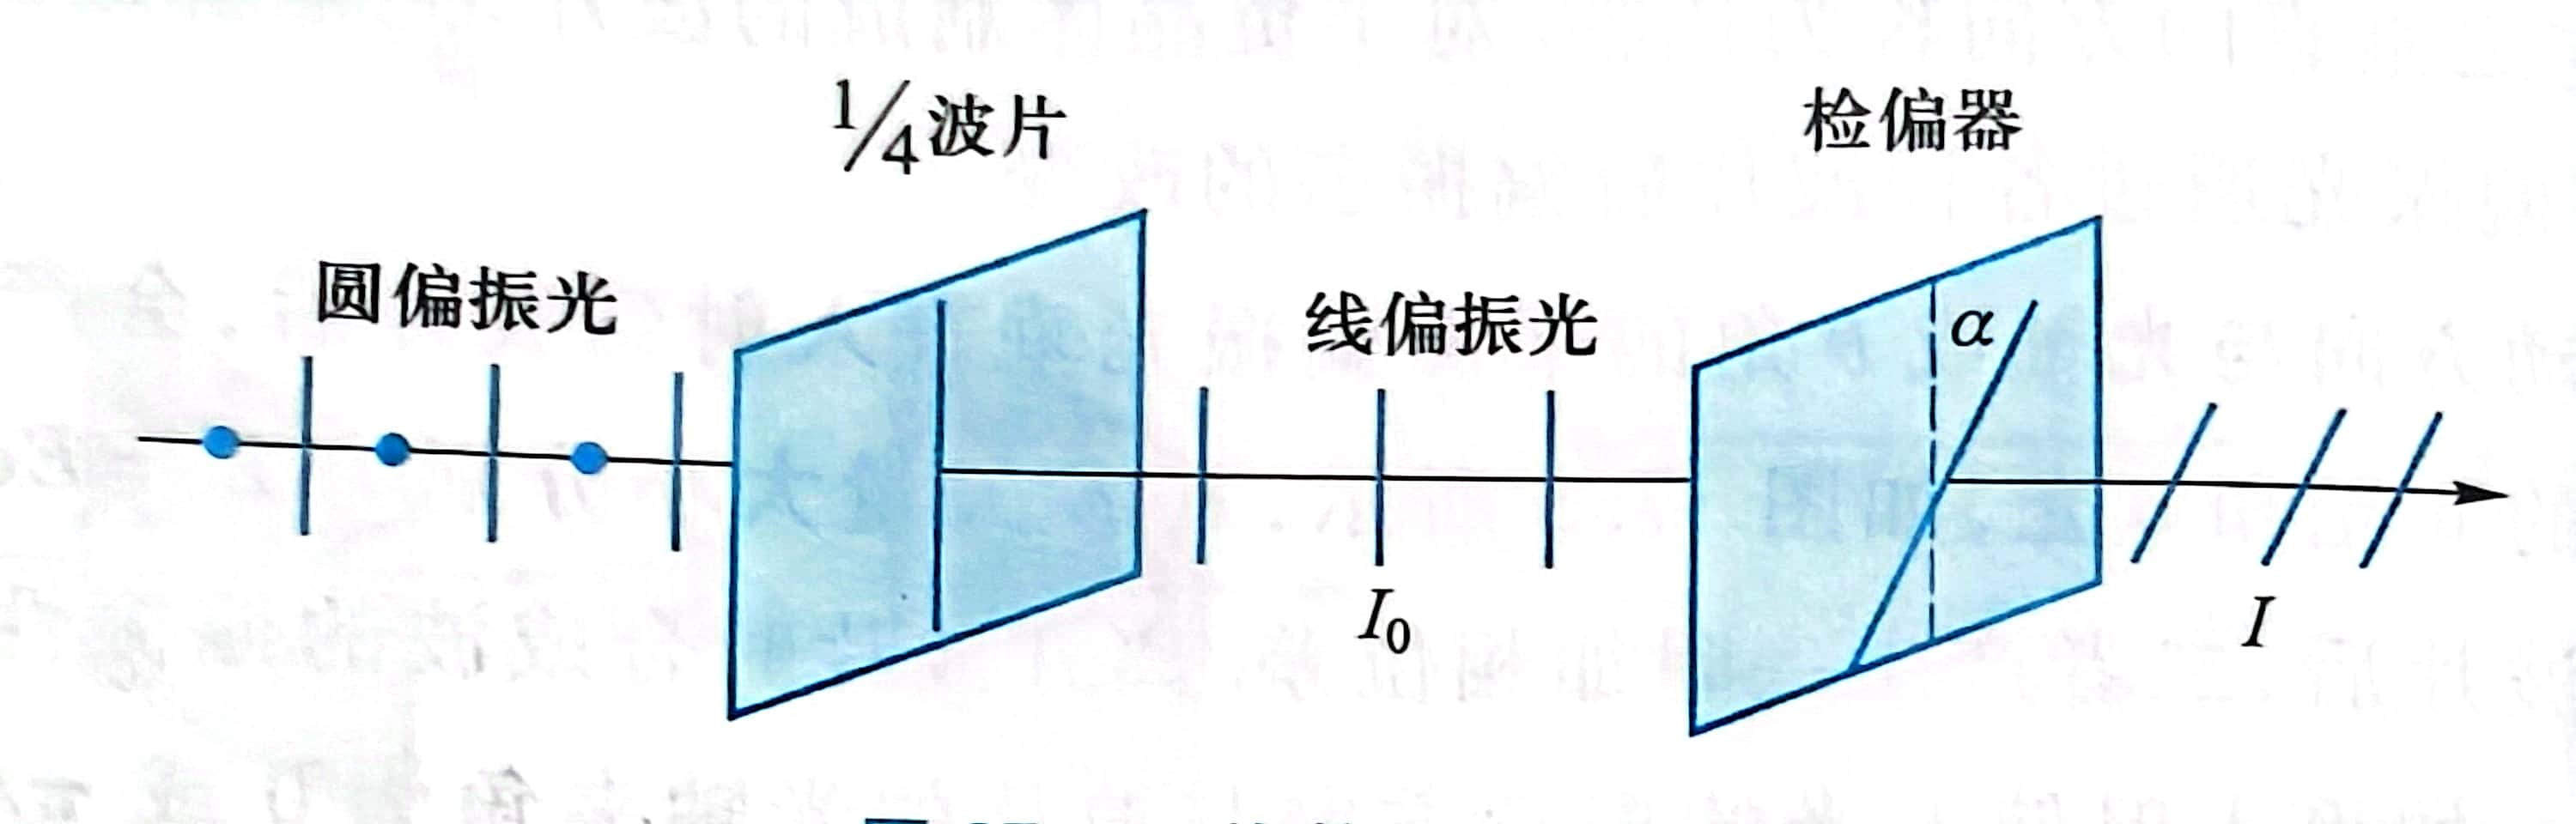
\includegraphics[width=0.8\textwidth,height=0.35\textheight]{jinyibujianbie.jpg}
    \caption{鉴别偏振光方法示意图2}
  \end{figure}

  \subsection{马吕斯定律}
  按照马吕斯定律,强度为h的线偏振光通过检偏器后,透射光的强度为
  \begin{equation}
    I=I_{0} \cos^{2} \alpha
  \end{equation}

  其中,$\alpha$为入射光偏振方向和检偏器偏振轴之间的夹角,$I_{0}$为检偏器透光部分与偏振光
  偏振方向平行时出现的出射光强,$I \leqslant I_{0}$。
  显然,当以光线传播方向为轴转动检偏器时,透射光强度1将发生周期性变化.当$\alpha = 0^{\circ}$时,透射光强度最大;当$\alpha=90^{\circ}$时,
  透射光强为最小值(消光状态),接近于全暗;当$0^{\circ} < \alpha < 90^{\circ}$时,
  透射光强度I介于最大值和最小值之间。因此,根据透射光强度变化的情况,可以区别线偏振光、自然光和部分偏振光。


\section{实验装置器材介绍}
半导体激光器,起偏器,检偏器,1/4波片,1/2波片,带广电接收器的数字式光功率计,光具座。


\section{实验内容及实验步骤}
  \subsection{激光器和起偏器的调整}
  实验采用波长为650nm的半导体激光器,它发出的是部分偏振光,为了得到线偏振光,如图\ref{shiyanguanglu}所示,需要在它前面加起偏器P,
  并放置接收器(检偏器A和波片C均先不要放置).转动起偏器P的偏振轴,使之与激光最强的线偏振分量方向一致,这时光功率计读数最大,透过起偏器P的线偏振光功率最大。
  
  \begin{figure}[H]\label{shiyanguanglu}
    \centering
    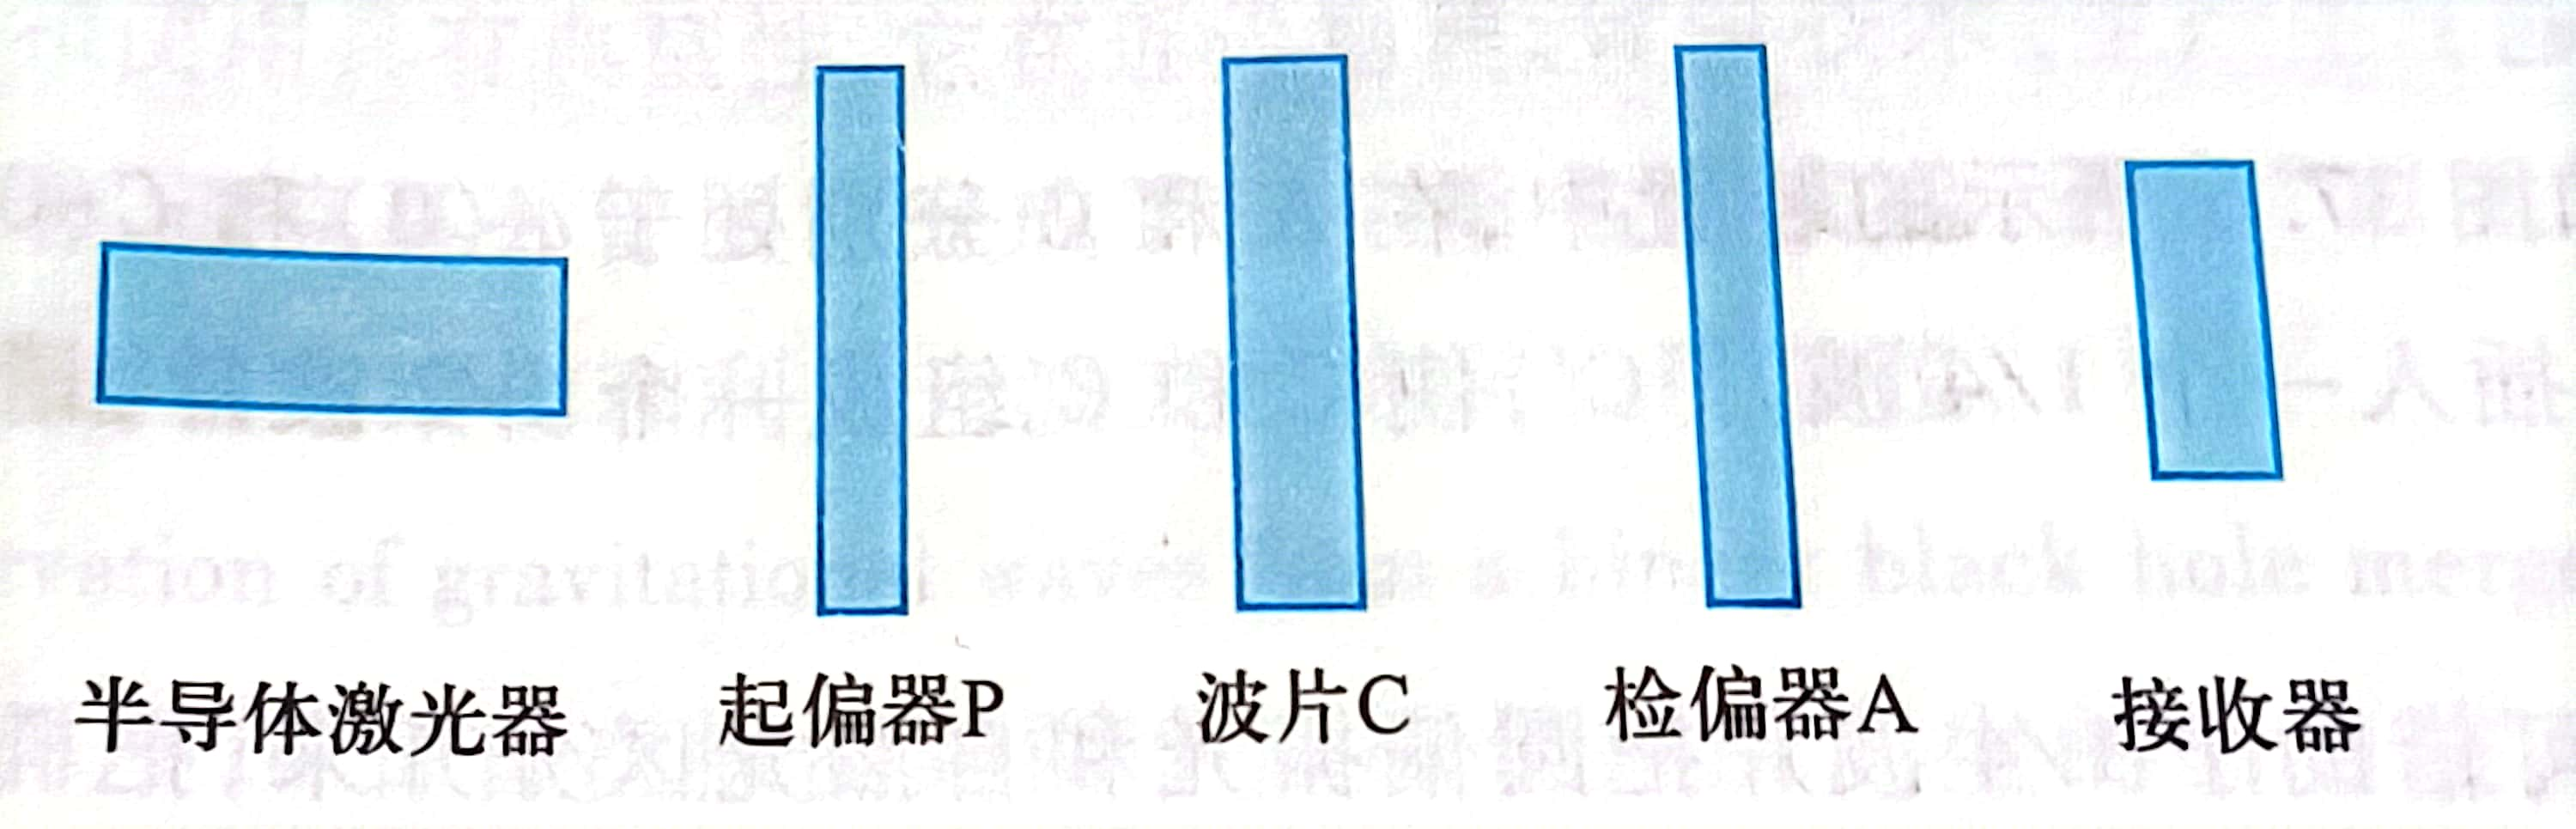
\includegraphics[width=0.8\textwidth,height=0.3\textheight]{shiyanguanglu.jpg}
    \caption{实验光路示意图}
  \end{figure}

  \subsection{验证马吕斯定律}
  在起偏器P与接收器之间加检偏器A,转动检偏器并测量出射最大光强,
  记为$I_{0}$,应反复多测几次,求平均值了和检偏器位置读数A(0).以A(0)作为$0^{\circ}$角.然后,
  每隔10°或15°,测量出射光强I.以$\ln (\cos \alpha)$为自变量,InI为因变量,对$\ln I-\ln(\cos \alpha)$进行直线拟合,
  求得函数$I=I_{0}\cos^{2}\alpha$中的n及相关系数$\tau$,以此证明马吕斯定律。

  \subsection{验证1/4波片的作用}
  转动检偏器A的偏振轴与激光的电矢量垂直至出现消光现象,记下检偏器A消光时的位置读数A(0).然后将1/4 
  波片C放在液片放置区,旋转C,使再次出现消光现象。
  这时 1/4 波片的快轴(或慢轴)与激光电矢量方向平行或垂直,记下1/4波片C消光时的位置读数C(0).
  旋转1/4 波片C,以改变其快(或慢)轴与入射线偏振光电矢量(即起偏器P透振方向)之间的夹角$\theta$。
  当$\theta$分别为15°、30°、45°、60°、75°、90°时,将A 旋转360°,观察光强的变化情况,记下二次最大值和最小值,
  并注意最大值和最小值之间检偏器A是否转过约90°,并由此说明1/4波片出射光的偏振情况。

  \subsection{圆、椭圆偏振光的鉴别}
  设计一个实验,要求用一块1/4波片产生圆偏振光或椭圆偏振光,再用另一块1/4波片使其出现线偏振光,记录下你的实验过程和实验结果。
\newpage

\section{实验原始数据}
\begin{figure}[H]
  \centering
  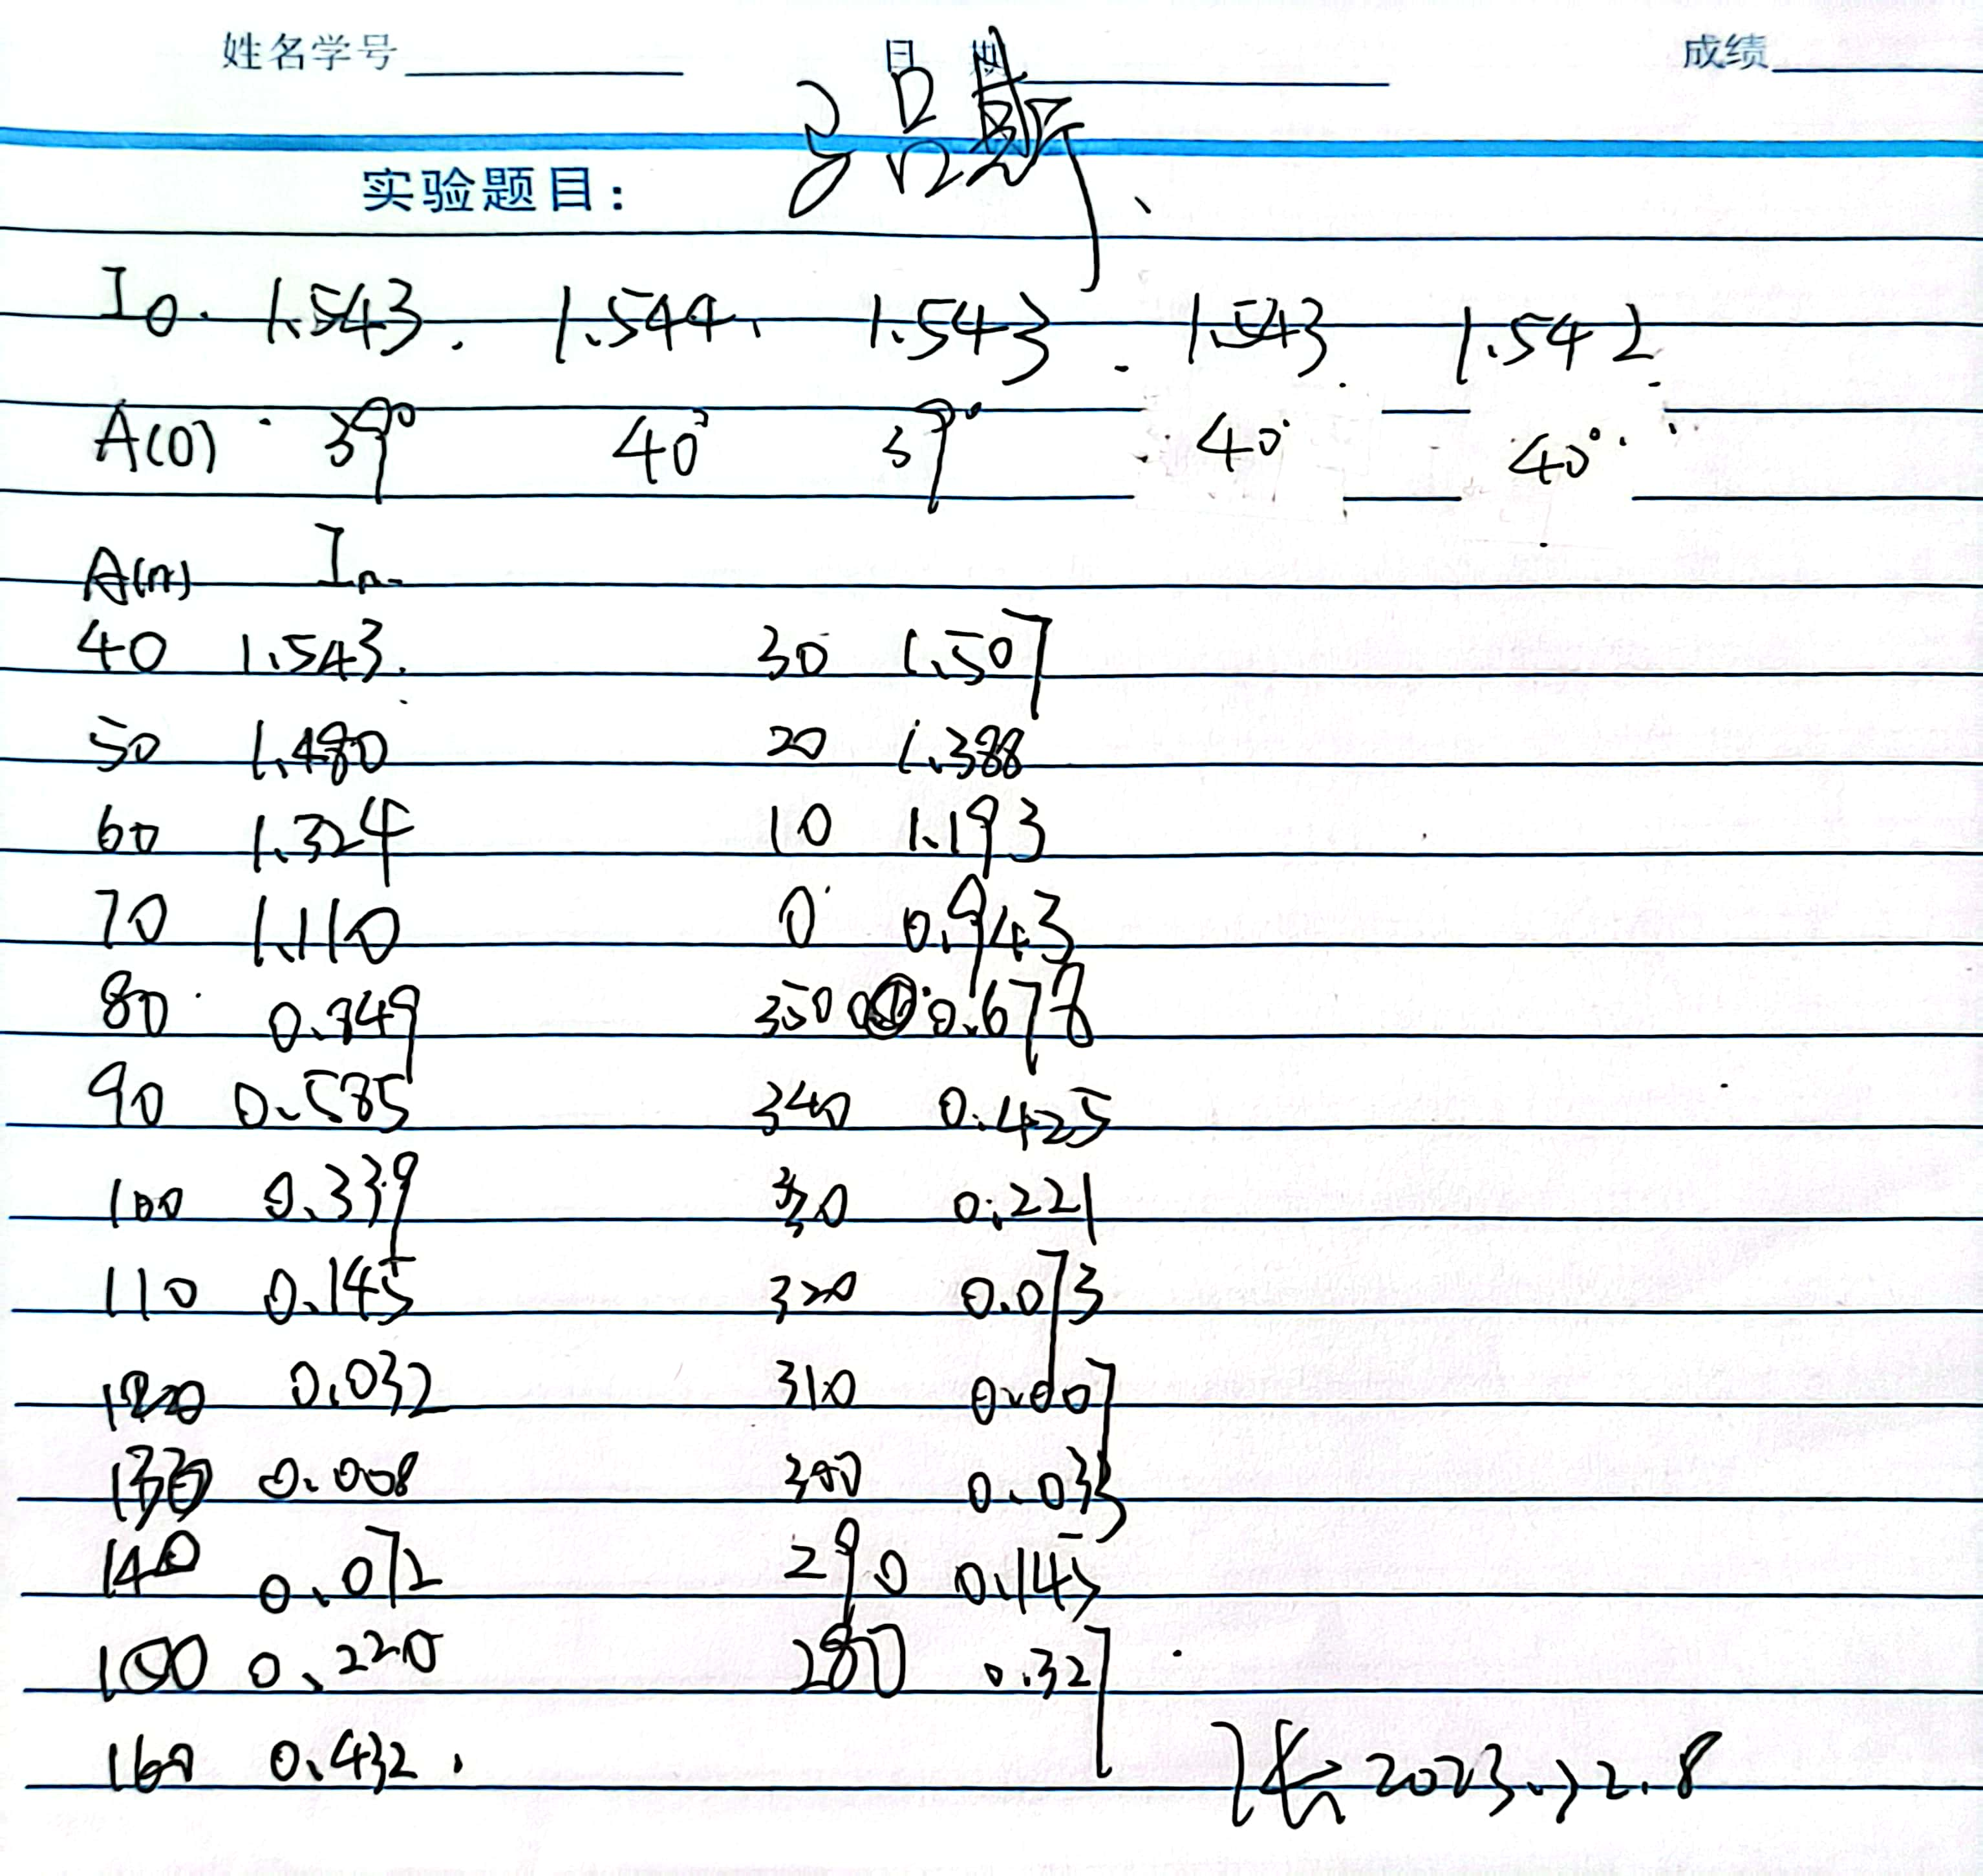
\includegraphics[width=0.9\textwidth,height=0.8\textheight]{yuanshishujv2.jpg}
  \caption{实验原始数据1}
\end{figure}
\newpage

\begin{figure}[H]
  \centering \label{shujv2}
  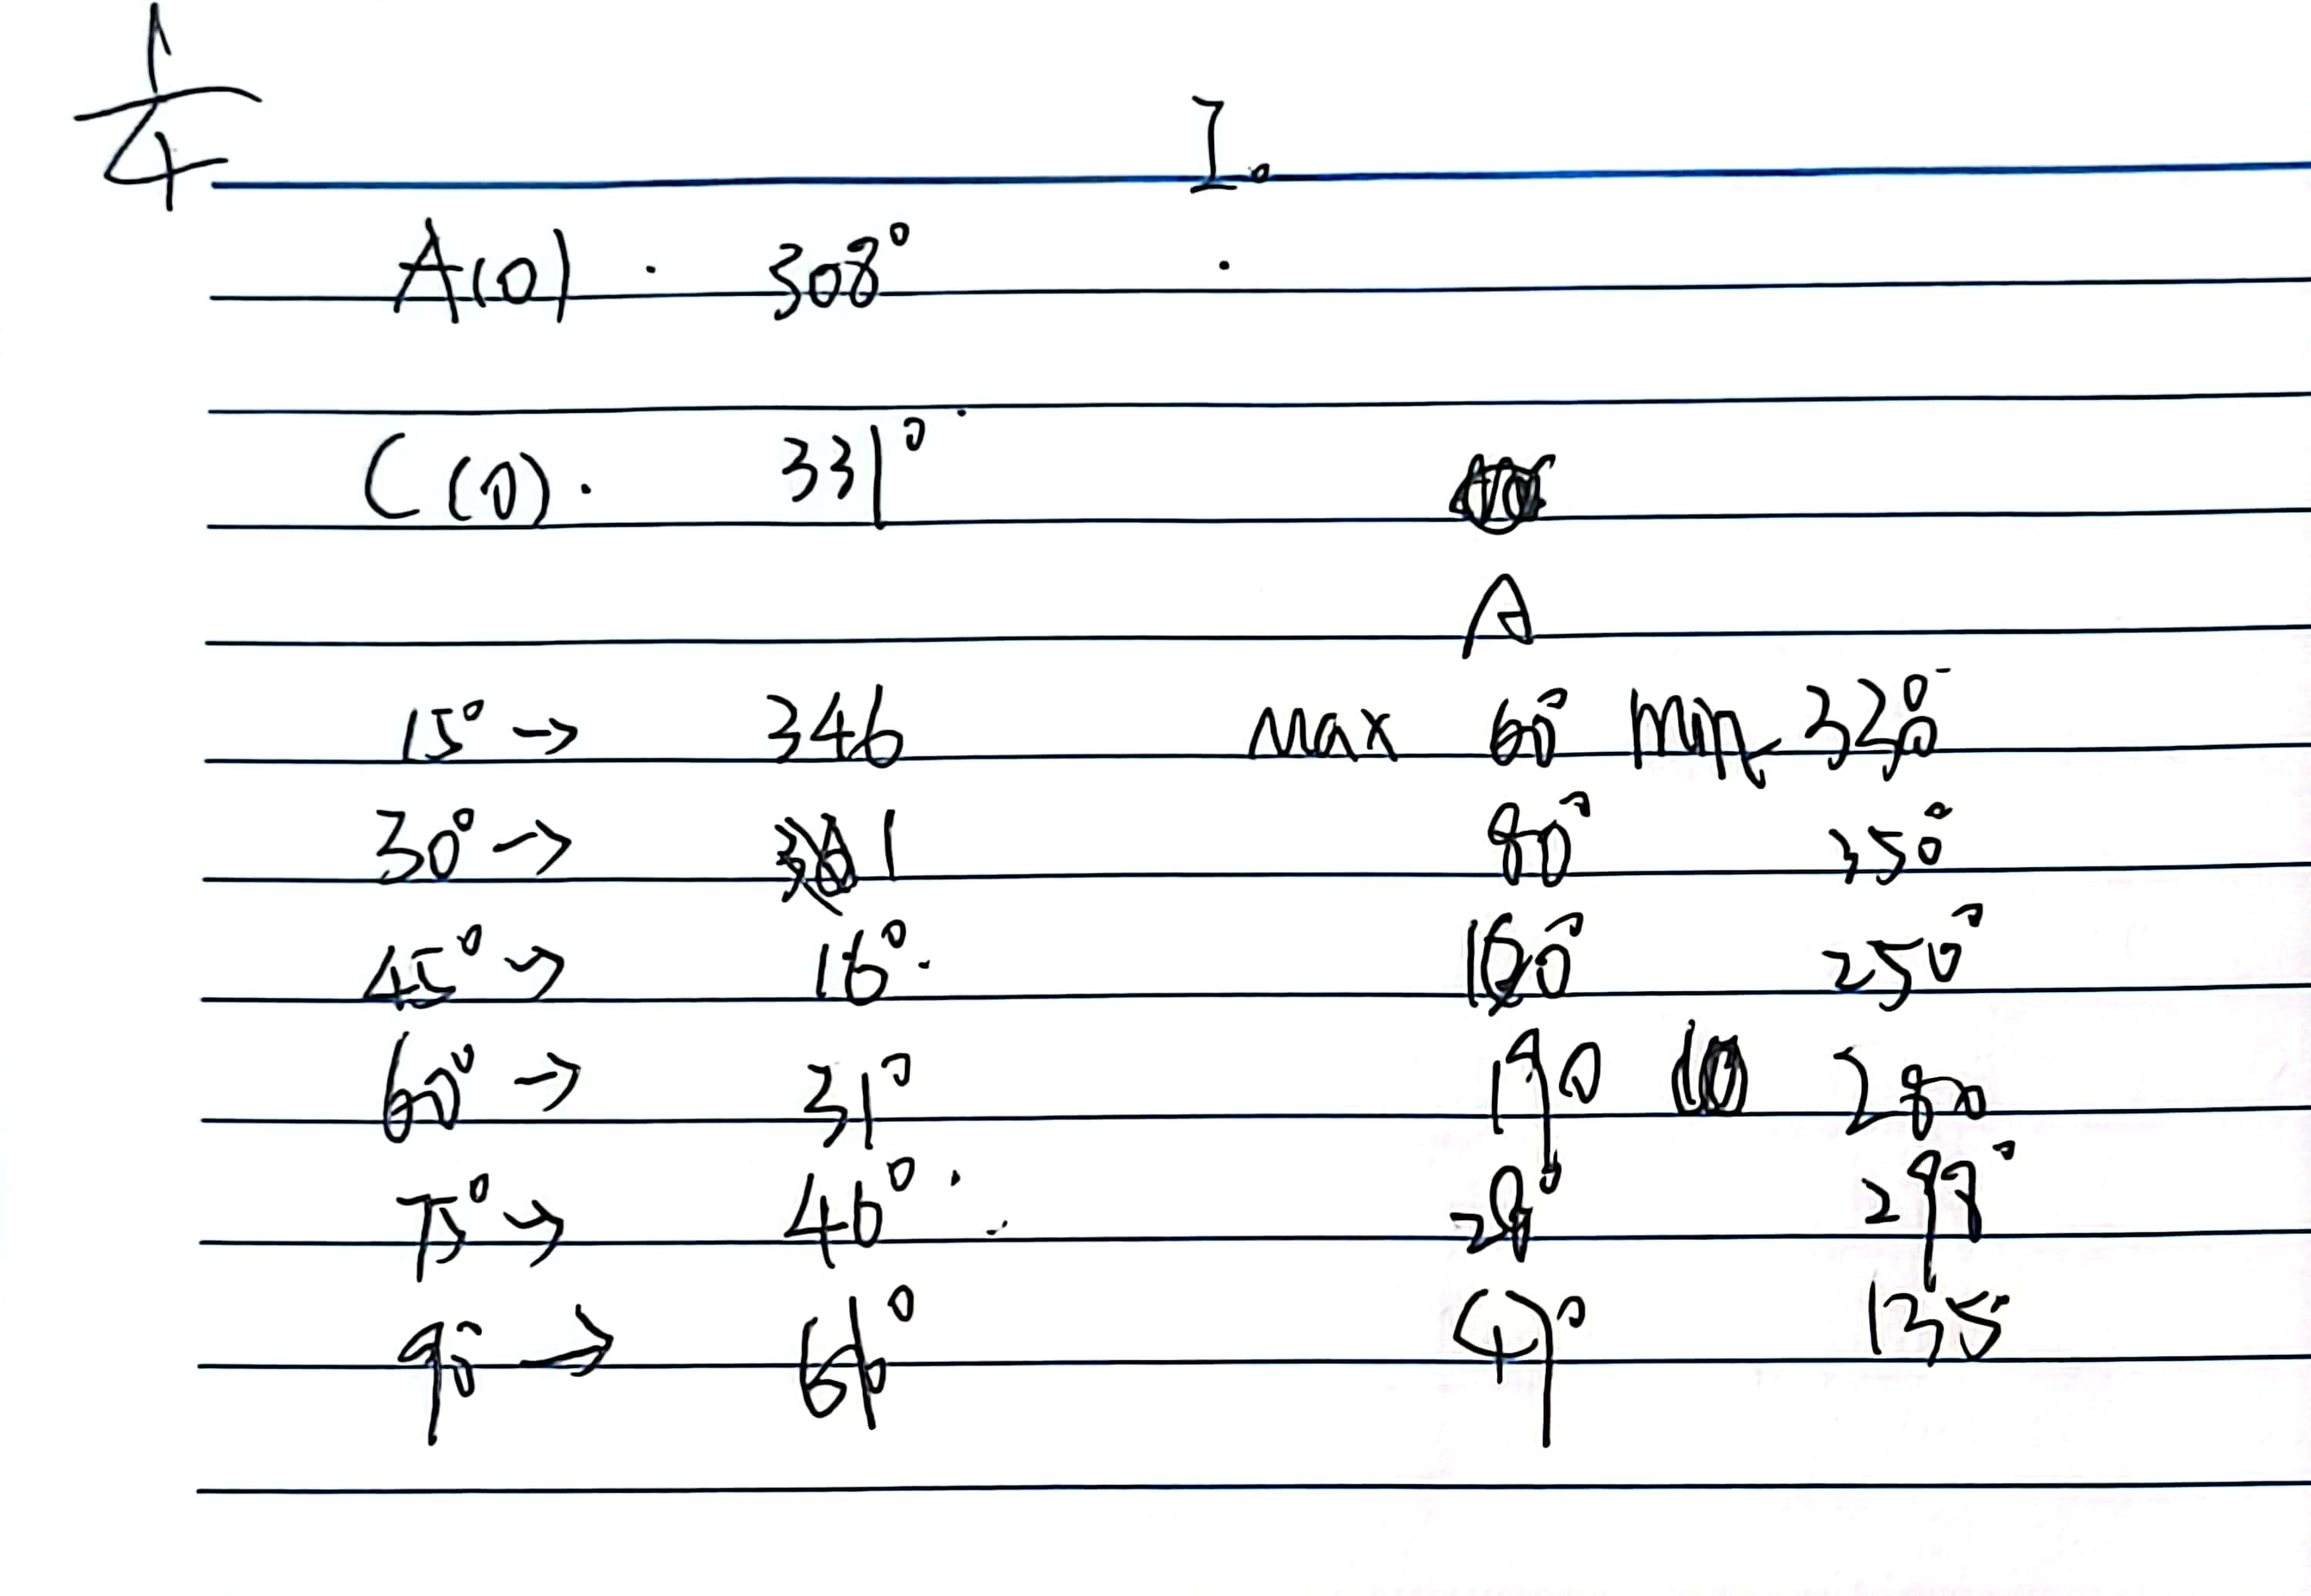
\includegraphics[width=0.7\textwidth,height=0.5\textheight]{yuanshishujv1.jpg}
  \caption{实验原始数据2}
\end{figure}
\newpage

\section{实验数据处理}
  \subsection{验证马吕斯定律}
  将实验获得的数据进行数据的处理后得到图像为图\ref{shiyanzuotu}所示。
  \begin{figure}[H]
    \centering \label{shiyanzuotu}
    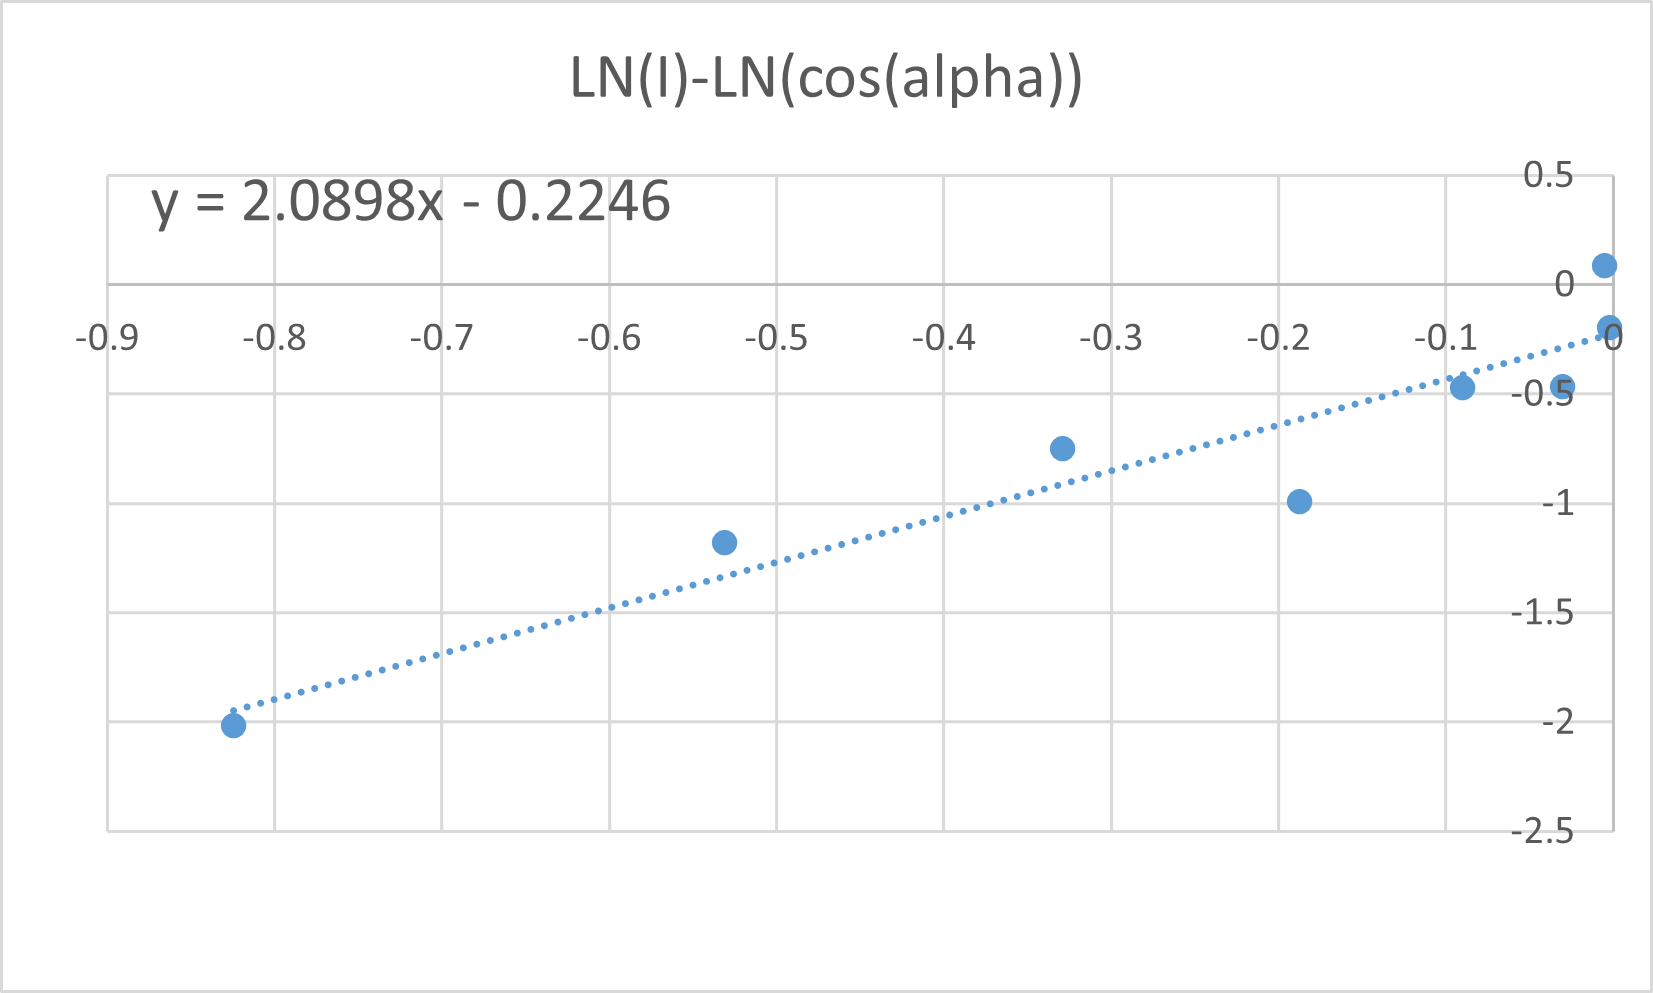
\includegraphics[width=0.8\textwidth,height=0.4\textheight]{zuotu.png}
    \caption{实验作图}
  \end{figure}

  最终可以看到得到的n为2.0898,和理论2的百分差为4.5\%。结果能够验证马吕斯定律。

  \subsection{验证1/4波片的作用}
  从原始数据,图\ref{shujv2}中可以看到每次转动后的最大值和最小值的差约等于90度,
  说明波片的作用能够产生线偏振光,产生最大值光和最小值光之间的相位差为90度。

  \subsection{圆、椭圆偏振光的鉴别}
  通过调节第一个1/4波片和起偏器的相位差,在通过第二个1/4波片调节,记录得到的相位,在图上做出
  角度和光强的极坐标图。最终得到实验结果。
\section{思考题}
  \subsection{思考题一}
  将第一个偏振片调节为相位差相差90度的位置,然后通过第二个1/4波片,这样就得到了和半波片相同的效果。

  \subsection{思考题二}
  可以。

  通过1/4的圆偏振光会变成线偏振光,而自然光还是自然光。还需要偏振片进行检测。

  而椭圆偏振光经过1/4会产生两次最大和消光,而部分偏振光不会有这样的现象,所以依旧可以。

\section{实验中个人的思考与感想}
  \subsection{对于实验个人观点}
  实验中需要的操作还是比较简单的,只要调节器材的旋转角度就可以了。观察的现象也比较明显,能够直接
  在仪器上读出。但是实验的原理还是比较复杂的,使用的器件结合产生的结果也会比较多样。

  最终得到的实验的结果还算理想。但是实验中还是有一些误差的存在,比如在读取角度的时候可能由于各种原因
  导致读数出现误差。

  \subsection{实验中的总结}
  实验验证了马吕斯定律,检验了1/4波片产生90度相位差,能将圆偏振转化为线偏振的性质,设计并实践了实验得到了
  圆偏振和椭圆偏振的结果。
\end{document}
